\documentclass{standalone}

\usepackage{tikz}

\usetikzlibrary{positioning, shadows, fit}

\begin{document}

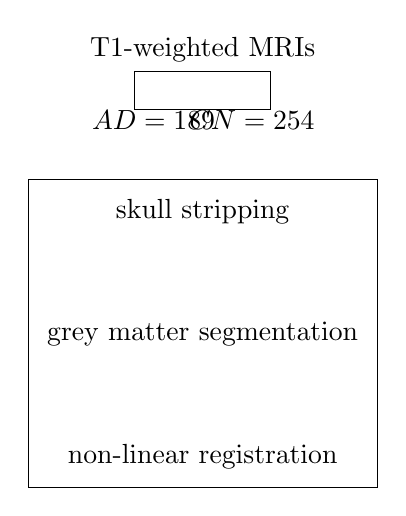
\begin{tikzpicture}
	\node[label=below:{$AD = 189$}] (ad) {};
	\node[label=below:{$CN = 254$}, right=of ad] (cn) {};
	\node[fit=(ad)(cn), label=above:{T1-weighted MRIs}, draw, rectangle] (adni) {};

	\node[below=of adni] (skull) {skull stripping};
	\node[below=of skull] (gms) {grey matter segmentation};
	\node[below=of gms] (im_reg) {non-linear registration};

	\node[fit=(skull)(gms)(im_reg), draw, rectangle] {};
\end{tikzpicture}

\end{document}
